\begin{appendix}

\chapter{Protocolo extracción y clonación de plásmidos}\label{Protocolo Plasmido}

Los plásmidos gentilmente donados por el laboratorio del Dr. Qin, fueron depositados en una gota sobre un papel y resaltado el contorno en circunferencia rotulada cada uno como $\alpha$IIb y $\beta$3, a partir de éstos se procedió con la extracción y clonación de cada uno por separado.


\begin{table}[]
  \begin{center}
  \centering
  \captionsetup{justification=centering}  % Center the caption
    \caption{Datos proteína fusión, segmentos transmembrana, MBP y TEV.}
    \label{tab:dat_proteina}
    \begin{tabular}{l l| l l }
      \toprule % <-- Toprule here

		$\alpha$IIb-Fusión & 49.41 kDa 	& $\alpha$IIb 	& 6.05 kDa \\ 
		{\Large{$\varepsilon$}}$_{\alpha \text{IIb-Fusión}}$ & 85830 M$^{\text{-1}}$cm$^{\text{-1}}$ & {\Large{$\varepsilon$}}$_{\alpha \text{IIb}}$ & 16500 M$^{\text{-1}}$cm$^{\text{-1}}$ \\
		$\beta$3-Fusión 	& 52.11 kDa 	& $\beta$3 	& 8.76 kDa \\
		{\Large{$\varepsilon$}}$_{\beta \text{3-Fusión}}$ & 83310 M$^{\text{-1}}$cm$^{\text{-1}}$ & {\Large{$\varepsilon$}}$_{\beta \text{3}}$ & 13980 M$^{\text{-1}}$cm$^{\text{-1}}$ \\
      \midrule % <-- Midrule here
      MPB & 42.49 kDa 	& TEV 	& 28.62 kDa \\ 
      
      
      \bottomrule % <-- Bottomrule here
    \end{tabular}
  \end{center}
\end{table}



    \begin{itemize}
     
     \item{Suspensión del plásmido en Buffer Trix}
      \begin{itemize}
        \item{Recortar media circunferencia de cada plásmido (tijeras estériles, limpiar con alcohol y flamear en fuego)}
        \item{Guardar el otro pedazo de papel a -20°C en bolsa ziploc}
        \item{Manipular con al semi-circunferencia con unas pinzas estériles, cortarlo en pedazos más pequeños}
        \item{Introducir los pedacitos en un eppendorf rotulado como corresponde ($\alpha$IIb ó $\beta$3)}
        \item{Agregar 50 µL de buffer Trix 50 mM pH 8. Evitar diluir mucho el plásmido}
        \item{Dejar 30 minutos en suspensión}
      \end{itemize}
    
    \item{Clonar los plásmidos}
      \begin{itemize}
        \item{Rotular dos viales eppendorf según corresponda, dejarlos en hielo}
        \item{Agregar a cada vial 100 µL de la cepa \emph{E. coli} DH5$\alpha$}
        \item{Tomar 10 µL del plásmido re-suspendido y transferirlos al vial que contiene la bacteria \emph{E. coli} DH5$\alpha$}
        \item{Tapar y dejar durante 30 minutos en hielo. Mientras espera, calentar baño termostático a 42°C}
        \item{Pasada la media hora, colocar los viales en el baño caliente durante 1 minuto y 30 segundos. Usar flotador de eppendorf}
        \item{Colocar de nuevo en el hielo durante 5 minutos}
        \item{Preparar el LB,  agregar 900 µL de LB a los eppendorf de $\alpha$IIb y $\beta$3 que contienen 100 $\mu$L de la cepa E. coli DH5$\alpha$ y los 10 µL de la suspensión de plásmido}
        \item{Llevarlos a 37°C durante 1 hora}
    \end{itemize}
    
    \item{Cultivo en caja de Petri}

     Utilizar 4 tubos ro, dos para el $\alpha$IIb y dos para el $\beta$3, donde tendremos una siembra diluida y una concentrada, es decir, de los tubos eppendorf anteriores (que contienen 900 $\mu$L de LB, 100 µL de la cepa E. coli DH5$\alpha$ y los 10 µL de la suspensión de cada plásmido), que tenemos después de someter a 37 °C durante una hora, ese líquido en primera instancia lo llamaremos “células diluidas”, luego centrifugamos a 4000 rpm/5 min (se va a observar un precipitado) y pipeteamos con mucho cuidado 800 $\mu$L los cuales desecharemos. Luego vamos a resuspender ese precipitado pipeteando lentamente y esa serán las “células concentradas”.

     \begin{itemize}
        \item{}
        \item{}
        \item{}
        \item{}
    \end{itemize}
        

Para el sembrado debemos tener las 4 cajas de Petri rotuladas como corresponde (diluida y concentrada tanto para $\alpha$IIb como $\beta$3). Utilizar perlas pequeñas para facilitar la “dispersión” de las células en el cultivo, para ello usar una “cucharita” que se flamea antes de sacar las perlas (entre 4 a 6 perlitas por caja de Petri). Evitar que las perlitas giren en círculos sobre las paredes de las cajas de Petri, la idea es que recorran todo el medio y no solo las paredes del medio.

Pipetear 100 µL de “células” y depositarlos sobre las perlitas, luego tapar la caja y agitar con la finalidad que se “depositen” células por todo el medio y obtener diferentes colonias de bacterias que se puedan aislar fácilmente. 


\item{Aislamiento de colonias}

De los cultivos que obtuvo anteriormente, seleccionar los que permitan aislar y/o identificar fácilmente una colonia. Las cuales se van a sembrar nuevamente en una caja de Petri con el mismo medio (LB con ampicilina 100 µg/mL; previamente secar). Para el caso específico se obtuvieron muchas colonias en las concentradas y se dificulta identificar algunas colonias, por lo tanto, seleccionamos las “diluidas” las cuales tenían colonias separadas unas de otras lo cual permite que “puncemos” con un palillo una colonia y luego sembrarla en el nuevo medio para aislar, y en medio de LB líquidos los cuales se guardarán en un freezer a -80 °C, más adelante. 
Sobre la tapa de los cultivos que mejor permite identificar colonias, encerrar cuatro colonias que son las que va a punzar con el palillo y posteriormente sembrar en el nuevo medio de cultivo.

     \begin{itemize}
        \item{}
        \item{}
        \item{}
        \item{}
    \end{itemize}


Además, los palillos que se usan en $\alpha$IIb$_{1,2}$ y $\beta$3$_{1,2}$ se introducen en los medios líquidos de LB, cada tubo de ensayo debe contener 2.5 mL LB con ampicilina [100 µg/mL]. Los palillos 3 y 4 se pueden desechar. La caja de Petri se incuba a 37 °C por más de 12 horas y los tubos de ensayo, con sus respectivas tapas se llevan a shaker a 37 °C por más de 12 horas.

NOTAS: 
    A. La idea de sembrar nuevamente en LB sólido es porque se obtienen colonias aisladas y una vez crezcan son las que se utilizarán para extraer los plásmidos y sembrarlos nuevamente, pero en la cepa de expresión.
    B. Los cultivos líquidos se hacen con la idea de que una vez se obtengan las células, se dejan en una solución de glicerol al 15$\%$ a -80 °C, y se usarán como “solución stock” cuando se necesite obtener células con el plásmido para expresar.

    C. Las cajas de los primeros 4 cultivos se guardan temporalmente en una nevera para tenerlas como respaldo por si pasa algo. 
    D. Para la preparación del LB con ampicilina, se debe solicitar a FACEMES el antibiótico, ellos entregan un eppendorf con 500 µL a una concentración de [100 mg/mL], el cual debe conservar siempre en hielo y dejar que se descongele en el hielo y una vez termine de usarlo, guardarlo a -20°C. El LB que se usa, es un frasco que viene rotulado como LB 50 mL; sino lo va usar todo procure preparar la cantidad necesaria y guardar bien el resto de LB sin antibiótico, ejemplo, si sólo necesita 20 mL de LB, y sabemos que la concentración de ampicilina debe ser [100 $\mu$g/mL], entonces le agregamos 20 $\mu$L de los 500 $\mu$L que le entrega FACEMES. 


\item{Guardar células en glicerol al 15$\%$ a -80°C}

De cada tubo de ensayo de cultivo líquido de LB, se extraen 500 µL y se vierten un tubo eppendorf, previamente rotulado y luego se le agredan 500 µL de glicerol al 30$\%$, es decir se obtiene 1 mL de “solución \textbf{stock de células}” al 15$\%$ de glicerol. Además, cada tubo se debe hacer por duplicado, y éstas son las muestras que se guardan a -80 °C. 
Antes de pipetear los 500 µL de células agitar bien el tubo y cuando agregue el glicerol, con la misma punta pipetear suave para que se “disuelva” bien el glicerol la solución.
Procurar tener todos los eppendorf tapados e ir trabajando uno por una por si de pronto salpica alguna gota de una cepa a un tubo diferente.

     \begin{itemize}
        \item{}
        \item{}
        \item{}
        \item{}
    \end{itemize}



\item{Minipreps y test de pureza}

Extracción de los plásmidos (Plus SV Minipreps DNA Purification System-Quick Protocol)
    A. Production of Cleared Lysate
De los cultivos del paso anterior, agitarlos un poco antes de pipetear de cada uno 1.5 mL y agregarlos en eppendorf rotulados como corresponde y dejar 5 minutos quieto. Al centrifugar colocar de la misma forma los tubos para que el pellet se forme siempre en el mismo lado de los tubos. Esto se hace porque en ocasiones el pellet no se ve a simple vista y si siempre colocamos los tubos de la misma forma, se sabrá en donde se encuentra y así uno cuando succione con la punta sabe que no debe tocar esa zona donde se supone que el pellet.

Cuando termine de centrifugar extraer de cada tubo la máxima cantidad posible del sobrenadante de cada tubo SIN TOCAR el pellet. Cambiar de punta cada vez que cambia de cepa. El sobrenadante se puede desechar. Aquí lo que se hace es obtener todas las células que contienen el plásmido.

Al terminar deberá obtener 4 tubos eppendorf con los correspondientes pellets, dos se guardan a -20 °C para tenerlos de respaldo por si algo o no se logra extraer el plásmido se parte de nuevo, pero de esas dos muestras que se guardan.
Se continua con el punto 2 del protocolo. Donde a los dos tubos se les agrega 250 mL de “Cell Resuspension Solution”. Tener mucho cuidado al pipetear de esta y las otras soluciones del protocolo, es decir, si al verter los 250 µL en uno de los tubos llega a tocar las paredes del mismo DEBE descartar esa punta y usar otra para pipetear de nuevo el reactivo correspondiente.

Una vez termine de agregar la solución de Resuspención, llevar cada tubo al vortex con la idea de que todo el pellet se disuelva; si necesita golpearlo con los dedos lo puede hacer. Observar que la solución que se obtiene es un poco “turbia” 

Punto 3: agregar 250 µL de “Cell Lysis Solution” a cada tubo e inmediatamente “invertir” el tubo suavemente unas 5-6 veces; debe observarse un cambio en la coloración, pasa de blanco-turbia a traslúcida. Lo que se hace en este paso es romper todas las células y sale el ADN que le da una “viscosidad” a la solución. Procurar no tener tanto tiempo en la mano el tubo después de agregar la solución de lisis.
Punto 4: Agregar 10 µL de “Alkaline Protease Solution”; en este caso como es una pequeña cantidad de solución, tratar de que con la misma punta que pipeteó los 10 µL, al agregarlos dentro de la solución y desechar la punta. Dejar 5 minutos en una gradilla a temperatura ambiente. Al agregar esta solución lo que se está haciendo es “desnaturalizar el ADN junto con las proteínas.
Punto 5: Agregar 350 µL de “Neutralization Solution”, casi que de inmediato se van a forman “grumos” blancos lo cual indica que se han “renaturalizado” proteínas, el ADN plasmático queda en la solución. 
Punto 6: Centrifugar a 13 mil rpm durante 10 minutos a 25 °C. 
Es muy importante no pipetear partes blancas; puede colocar dos puntas en la micropipeta para que se facilite y succione mejor el líquido. El eppendorf de donde sacamos el líquido, se desecha en una bolsa roja. 

    B. Binding of Plasmid DNA
Punto 7-8: El líquido que se pipetea se vierte en la columna o tubo de membrana “Spin Column” con su correspondiente tubo colector (puede ser un eppendorf estéril.
Punto 9: Centrifugar por un minuto a 13 mil rpm a temperatura ambiente. El contenido del líquido del tubo colector se descarta. Tener mucho cuidado al retirar la Spin Column de no tocar las paredes internas y mucho menos la membrana.
    C. Washing
Punto 10: Para el lavado se agregan 750 µL de “Wash Solution” 

Paso extra!!
Antes de la elución cambiar el tubo colector y colocar la Spin Column en otro tubo colector que esté limpio, seco y sin EtOH o puede usar un eppendorf y soportar la Spin Column en este y centrifugar así sin nada por 2 minutos a 13 mil rpm. La idea es que no quede nada de EtOH en la columna.

    D. Elution
Lo que se hará en éste paso es desprender el plásmido que quedó en la membrana, por lo tanto, se debe buscar un eppendorf totalmente estéril y nuevo, los cuales deben estar rotulados como corresponde. 
Punto 13: Transferimos la Spin Column como se hizo en el paso extra.
Punto 14: Agregar 100 µL de “Nuclease-Free Water” o la mejor calidad de agua ultra pura que tenga. Procurar en este paso verter el agua cerca de la membrana, pero sin tocarla y desechar la punta que se usó. Dejar 2 minutos en reposo como para que se absorba bien el agua y luego centrifugar a 13 mil rpm por 1 minuto con la tapa abierta.


     \begin{itemize}
        \item{}
        \item{}
        \item{}
        \item{}
    \end{itemize}
\end{itemize}

\chapter{Protocolo expresión, lisis y purificación de proteína fusión}\label{Protocolo_Fusion}
El siguiente protocolo se realizó para expresar 4L de cultivo de proteína fusión a partir del stock\textbf{stock de células} de cada péptido.

\subsection{Expresión}

\begin{itemize}
    \item{Pre-inóculo en cepa \ac{ecoli} BL21(DE3)}
    \begin{itemize}
        \item{Tomar un frasco de agar \ac{lb} de 100 mL}
        \item{Suplementar con 100 µL de ampicilina stock [100 mg/mL]}
        \item{Sacar uno de los \textbf{stock de células} en hielo}
        \item{Usar punta (tip) amarillo para raspar y sacar células y arrojar tips al frasco}
        \item{Dejar overnight a 37°C toda la noche con agitación constante}
    \end{itemize}

    \item{Crecer células e inducir con IPTG}.
    Para crecer las células se usaron Erlenmeyers de capacidad para 3L pero se agregaron 1L de \ac{lb} en cada uno suplementado con 1.0 mL de ampicilina [100 mg/mL].
    \begin{itemize}
        \item{Tomar 25 mL del precultivo y agregarlo a cada Erlenmeyer}
        \item{Crecer a 37°C con agitación constante hasta obtener una \ac{DO$_{600}$} entre 0.7-0.8 ($\approx$ 7 horas)}
        \item{Agregar 1.0 mL de IPTG 1 M, [1.0 mM]$_{final}$}
        \item{Fortificar ampicilina, agregando 500 µL a cada cultivo}
        \item{Dejar nuevamente a 37°C con agitación por 5 horas}
    \end{itemize}

        \item{Centrifugar medios}
    \begin{itemize}
        \item{Trasvasar el cultivo a los frasco de polipropileno Nalgene (capacidad de 500 mL). Verificar que todas tengan el mismo peso}
        \item{Colectar células por centrifugación a 4°C, 4500 \ac{rpm} durante 30 minutos}
        \item{Descartar el sobrenadante}
    \end{itemize}
    Después de obtener un \textbf{pellet} (precipitado) en cada frasco, juntar en 2 falcón de 50 mL y guardar a -20°C si va lisar pronto, de lo contrario guardar a -80°C, congelando previamente con nitrógeno líquido.
\end{itemize}

\section{Lisis de células}
Seguimiendo de la proteína por geles de \ac{SDS-PAGE}, parte de la proteína fusión fue a cuerpos de inclusión, por lo tanto, para obtener la mayor cantidad de proteína se realizó un rompimiento de células exhaustivo aplicando tres métodos de lisis: ciclos frío-calor, incubación con Lisozima-ADNasa, (Freeze/Thaw) y alta presión (homogeneizador Emulsiflex).


\begin{itemize}
\item{Ciclos frío-calor}
     \begin{itemize}
         \item{Resuspender cada pellet en 25 mL buffer de lisis \ac{pbs} 20 mM, 300 mM NaCl y 20 mM imidazol} + Triton X-100 [0.25$\%$]$_{final}$ (v/v)
        \item{Congelar muestras con nitrógeno líquido y dejar a -80°C por 2 horas}
        \item{Descongelar en un baño de agua a temperatura ambiente}
        \item{Repetir proceso al menos 3 veces}
    \end{itemize}
\end{itemize}

\begin{itemize}
\item{incubación con Lisozima-ADNasa}
     \begin{itemize}
        \item{Agregar inhibidor de proteasa \ac{pmsf} a concentración [1 mM]$_{final}$}
        \item{Agregar lisozima bovina [5 mg/L cultivo]$_{final}$}
        \item{Agregar DNAsa [0.5 mg/L cultivo]$_{final}$}
        \item{Agregar EDTA [1.0 mM]$_{final}$}
        \item{Dejar a 4°C con agitación en rotor overnight}
    \end{itemize}
\end{itemize}

\begin{itemize}
\item{Homogeneizador Emulsiflex}
     \begin{itemize}
        \item{Pasar cada muestra al menos 4 veces por el Emulsiflex}
        \item{Fijarse visualmente en la densidad y flujo al salir del Emulsiflex}
        \item{Después de los 4 ciclos, la muestra debe ser casi un líquido fluido}
    \end{itemize}

Finalmente las muestras fueron centrifudas a 9500 \ac{rpm} por 30 minutos a 4°C (Eppendorf™ Centrifuge 5804R), conservando el \textbf{sobrenadante}. 
\end{itemize}

\section{Purificación por \ac{fplc}}

\begin{itemize}
    \item{Elución}
     \begin{itemize}
        \item{Equilibrar la columna con buffer A (el mismo de lisis)}
        \item{Cargar el contenido de 2L de cultivo; si carga más podría sobre saturar la columna. Usar bomba peristáltica}
        \item{Lavar con 10 \ac{cv} pasando buffer A. NO DESCARTAR ya que por geles \ac{SDS-PAGE} se observó que había proteína fusión, por lo tanto, se pasó después nuevamente por la columna}
        \item{Llevar columna al \"{A}KTA y pasar otros 10-20 mL de buffer A para obtener una buena base de linea en el cromatograma}
        \item{Eluir con buffer B, gradiente de imidazol de 20 a 400 mM (\ac{pbs} 20 mM, NaCl 300 mM, 400 mM imizadol)}
        \item{Colectar fracciones}
    \end{itemize}
\end{itemize}

\section{Concentrar y desalar proteína fusión}
Antes de cuantificar la concentración de cada proteína fusión, se procedió a concentrar todo el contenido de las fracciones colectadas en centricones Amicon Ultra-15 Centrifugal con 30 kDa  cutoff y cambiar de buffer en columnas PD-10 Desalting (GE Healthcare).

\begin{itemize}
    \item{Concentrar}
     \begin{itemize}
        \item{Lavar centricones de cuttoff 30 kDa agua Milli-Q}
        \item{Juntar todas las fracciones colectadas}
        \item{Agregar igual cantidad de volumen a cada Amicon}
        \item{Centrifugar a 4500 \ac{rpm} a 4°C por $\approx$ 20 minutos}
        \item{Conservar el contenido retenido}
        \item{Repetir pasos hasta concentrar toda la muestra}
    \end{itemize}

    \item{Desalar}
     \begin{itemize}
        \item{Equilibrar columna con buffer C (\ac{pbs} 20 mM, NaCl 150 mM y 7.5$\%$ glicerol (vol/vol) pH 7.4)}
        \item{Cargar muestra y eluir hasta casi sequedad}
        \item{Agregar buffer C, eluir}
        \item{Repetir hasta pasar toda la muestra previamente concentrada}
    \end{itemize}
    \item{Cuantificar por  espectrofotometría \ac{uv}}
    \item{Fraccionar en eppendorff y guardar a -20ºC/-80ºC}
Para más detalles consultar la ficha técnica en el siguiente link:  \url{https://www.scientificlabs.co.uk/handlers/libraryFiles.ashx?filename=Manuals_1_17085101_A.pdf}
\end{itemize}

\section{Protocolo de clivaje y diálisis}\label{Protocolo_TEV}

Tener en cuenta que la relación \ac{tev}:proteína es 1:30 mol a mol, por lo tanto, calcular bien la cantidad proteasa a usar según las concentraciones de TEV - proteína.

Ejemplo, si TEV = [1.0 mg/mL] y proteína [1.0 mg/mL], entonces,

$
\left( \frac{1.0 \, mg}{mL}*\frac{1 \,  g}{1000 \, mg}*\frac{1\,  mol\,  \alpha IIb}{49400\,  g}*1 \, mL \right)*10^9= 20.24 \;nmoles \;  \alpha IIb
$


$
\frac{20.24}{30} = 0.67
$

$
0.67\, nmol \,TEV*\frac{1 \,mol}{10^9 \,nmol}*\frac{28619.5 \,g}{1 \,mol\, TEV}*\frac{1000 \,mg}{1 \,g}*\frac{1000\, \mu L}{1\, mL} = 19.17 \; \mu L 
$
\begin{itemize}
    \item{Clivaje con TEV}
    \begin{itemize}
        \item{Descongelar las muestras de proteína}
        \item{Agregar \ac{dtt} [1.0 mM]$_{final}$}
        \item{Agregar 19.17 µL de TEV a cada vial}
        \item{Tapar y agitar suave}
        \item{Dejar a 30ºC por al menos 48 horas}
        \item{Centrifugar todos los viales a 13 mil \ac{rpm} por 10 minutos a temperatura ambiente}
        \item{Recuperar el \textbf{sobrenadante}}
        \item{Juntar todos los sobrenadantes y }
        \item{Concentrar en   Amicon Ultra-15 Centrifugal con 3 kDa  cutoff, 4500 \ac{rpm} a 4°C por $\approx$ 40 minutos}
    \end{itemize}

    \item{Diálisis}
    \begin{itemize}
        \item{Lavar las membranas con EDTA y bicarbonato de sodio a 60ºC por 5 minutos}
        \item{Pasar flujo de agua Milli-Q por la membrana o dejar en remojo con agitación suave por 2 horas}
        \item{Cerrar uno de los estremos, verificar que este bien sellado}
        \item{Agregar la muestra evitando dejar aire pero lo suficiente para sellar el otro extremo}
        \item{Colocar membranas en beaker de al menos 1L con agua Milli-Q
        }
        \item{Dejar 4ºC con agitación suave. Realizar dos cambios de agua al menos dos veces cada 8 horas}
        \item{Remover toda la muestra incluyendo el precipitado y pasarlo a eppendorf}
        \item{Centrifugar todos los viales a 13 mil \ac{rpm} por 10 minutos a temperatura ambiente}
        \item{Separar cuidadosamente el \textbf{pellet}}
        \item{Juntar los pellets en falcón de 50 mL y resuspender en buffer (fase móvil A (H$_{2}$O:\ac{acn} 60\%/\%40, vol/vol, \ac{tfa} 0.01\% vol/vol)}
        \item{Calentar a baño María $\approx$ 40°C para facilitar la solubilización}
        \item{Fraccionar en eppendorf y centrifugar todos los viales a 13 mil \ac{rpm} por 20 minutos a temperatura ambiente}
        \item{Tomar sobrenadante, juntar nuevamente y filtrar con membranas PVDF 0.45 µm (Durapore Merck). Esto para proteger al máximo la columna del \ac{hplc}}
    \end{itemize}

    
\end{itemize}


\chapter{Protocolo \ac{hplc}}\label{Protocolo_HPLC}
Tenga presente que los solventes deben ser grado \ac{hplc}, el agua Milli-Q se debe filtrar con membranas PVDF 0.22 µm y desgasificar. Se recomienda seguir los cuidados de la columna según el manul del usuario disponible en: \url{https://vneshbiotorg.ru/upload/welch/use-and-maintainance-of-hplc-column-welch%20materials.pdf}.

\begin{itemize}
    \item{Purgar equipo y equilibrar columna}
     \begin{itemize}
        \item{Lavar y purgar bombas y loop del  \ac{hplc} con agua y luego con la fase móvil A}
        \item{Equilibrar columna. Fijarse si esta en \ac{meoh} debe hacer el cambio con los cuidados necesarios de gradiente y flujo}
        \item{Correr al menos 10 \ac{cv} de fase móvil A a 1.0 mL/min a 40°C}
        \item{Verificar que la presión no sobrepase los 210 bar. Si los supera bajar el flujo}
    \end{itemize}
\end{itemize}

\begin{itemize}
    \item{Inyectar y correr muestra}
     \begin{itemize}
        \item{Cargar 1 mL en el loop de la muestra previamente solubilizada y filtrada}
        \item{Iniciar cromatografía con el gradiente especificado en la Tabla \ref{hplc_gradiente}}
        \item{Colectar todas las fracciones con muestran señal en el \ac{uv} a 280 nm distinguiendo en los diferente picos cromatográficos, es decir, que se resuelvan bien en el tiempo. El pico de los péptidos corresponde al \ac{tr} de 40-45 minutos}
        \item{Equilibrar de nuevo y repetir proceso hasta pasar toda la muestra}
        \item{Lavar bien la columna y el equipo \ac{hplc}}
    \end{itemize}
\end{itemize}

\begin{itemize}
    \item{Liofilizar y remover \ac{tfa}}
    Anteriormente se mencionó colectar las fracciones correspondientes a los picos del cromatograma que se resuelven bien entre ellos, esto para hacer seguimiento por geles \ac{SDS-PAGE}, sin embargo, como ya se dijo el pico correspondiente a los péptidos puros sale a los 40 minutos.
     \begin{itemize}
        \item{Juntar todas las fracciones del minuto 40 en un balón de destilación}
        \item{Llevar a un rotaevaporador hasta sequedad}
        \item{Pasar balón a una línea de Schlenk o rampa de vacío con doble trampa de nitrógeno líquido
        \item{Realizaron entre 3-4 lavados con \ac{acn}:H$_{2}$O:A. acético} al 60\%:20\%:20\% (vol/vol) para remover el \ac{tfa}}
        \item{Finalmente el péptido se resuspendión en \ac{acn}:H$_{2}$O 67\%:33\% (vol/vol) y se verificó la presencia del \ac{tfa} a los 1671 cm$^{-1}$}
    \end{itemize}
\end{itemize}



\chapter{Protocolo monocapas}


\begin{itemize}
    \item{}
     \begin{itemize}
        \item{}
        \item{}
        \item{}
        \item{}
    \end{itemize}
\end{itemize}

\begin{itemize}
    \item{}
     \begin{itemize}
        \item{}
        \item{}
        \item{}
        \item{}
    \end{itemize}
\end{itemize}


Los experimentos de monocapas se realizaron en una unidad de control de Monofilmmeter (con Film Lift, Mayer Feintechnique, Alemania). La presión superficial ($\pi$) se midió usando el método de Wilhelmy con una placa Platinized-Pt y el potencial superficial ($\Delta$V) se detectó mediante el uso de una placa ionizante de $^{241}$Am. Los datos fueron registrados de forma continua y simultánea con un registrador X-YY de doble canal. El área superficial total de la cubo de Teflón fue de 80 cm$^2$ con capacidad de 75 mL volumen para la subfase (PBS 20 mM, NaCl 100 mM a pH 7.4). Para los péptidos puros se evaporó el solvente ACN:H$_2$O con flujo de nitrógeno N$_{2 (g)}$ y se realizaron al menos 3 lavados con CHCl$_3$:MeOH 2:1 (vol/vol). La monocapa del péptido puro se formó directamente sembrando 0.5 nmoles  solución CHCl$_3$:MeOH  en la subfase usando un jeringa Hamilton. Tanto la isoterma del lípido puro como para las mezclas con péptidos se procedió de forma similar y se esperó por 8 minutos antes de empezar la compresión dar tiempo a la evaporación del solvente y posteriormente se empezó a comprimir a razón fija de \hl{xx} cm$^2$/min. Antes de sembrar muestras se realizaron los respectivos controles, para la superficie limpia y los disolventes de las muestras, en donde no se observó actividad superficial. Cada experimento se realizó por triplicado de forma independiente y se prepararon soluciones stock frescas de cada lípido cerca al momento de utilizarse.

Se realizaron ciclos de compresión-expansión, inicialmente las barreras se fijaron en 60 cm$^2$, se inició la compresión hasta llegar a los $\approx$ 13 cm$^2$ y se expandió hasta los $\approx$ 60 cm$^2$ y así se repitió tres veces para cada muestra.



%%%%%%%%%%% Figura %%%%%%%%%%%%
\begin{figure}[]
    \centering
	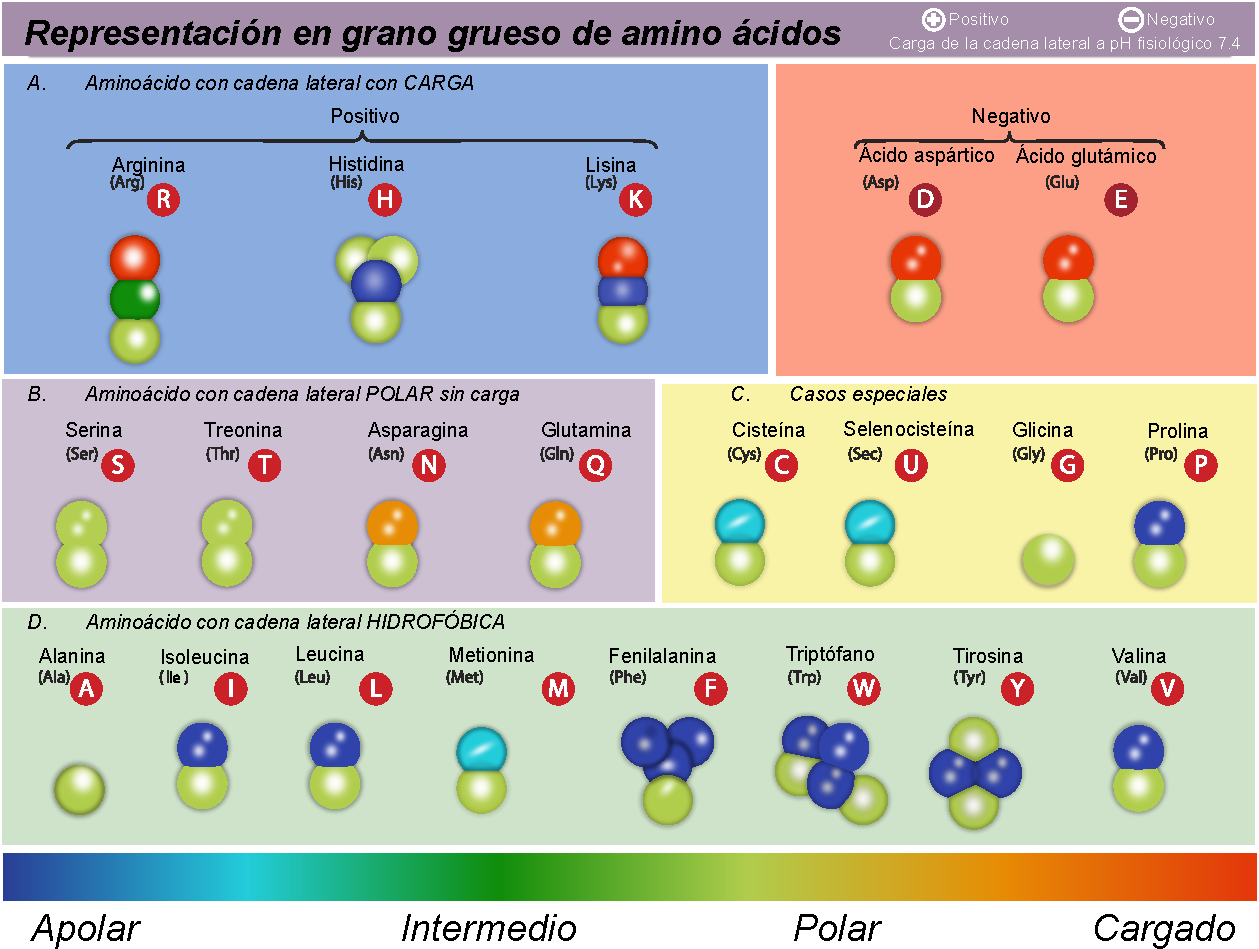
\includegraphics[width=1\linewidth, height=0.99\textheight, keepaspectratio]{fig/04_anexos/cg_aa.pdf} 
\caption[Representación en grano grueso de de los 21 amino ácidos]{Representación en grano grueso de de los 21 amino ácidos}
        \index{cg_aa}
    \label{tab:tabla_cg_aa}
\end{figure}
%%%%%%%%%%%%%%%%%%%%%%% Fin %%%%%%%%%%%%%%%%%%%%%%%%




\subsection{Campo de fuerza MARTINI}



%%%Tabla tomada de la tesis: lipid_protein_interaction...
% Please add the following required packages to your document preamble:
% \usepackage{booktabs}
% \usepackage[table,xcdraw]{xcolor}
% Beamer presentation requires \usepackage{colortbl} instead of \usepackage[table,xcdraw]{xcolor}
\begin{table}[]
\centering
\caption{Mapeo de la cadena lateral de amino ácidos con el campo de fuerza MARTINI v2.1. Partículas en grano grueso (CG)}
\label{tab:cg_particles}
\begin{tabular}{@{}ll@{}}
\toprule
\rowcolor[HTML]{EFEFEF} 
\multicolumn{1}{l}{\cellcolor[HTML]{EFEFEF}Cadena lateral} & \multicolumn{1}{l}{\cellcolor[HTML]{EFEFEF}Partícula GG} \\ \midrule
Leu/Ile  & C1              \\
Val/Pro  & C2              \\
Met/Cys  & P1              \\
Ser/Thr  & P5              \\
Gln      & P4              \\
Asp$^\text{--1}$ & Qa              \\
Asp$^0$  & P3              \\
Glu$^\text{--1}$ & Qa              \\
Glu$^0$  & P1              \\
Arg$^\text{--1}$ & N0-Qd           \\
Arg$^0$  & N0-P4            \\
Lys$^\text{--1}$ & C3-Qd           \\
Lys$^0$  & C3-P1           \\
His      & SC4-SP1-SP1     \\
Phe      & SC4-SC4-SC4     \\
Tyr      & SC4-SC4-SP1     \\
Trp      & SC4-SP1-SC4-SC4 \\ \bottomrule
\end{tabular}
\end{table}



%%%%%%%%%%% Figura %%%%%%%%%%%%
\begin{figure}[]
    \centering
	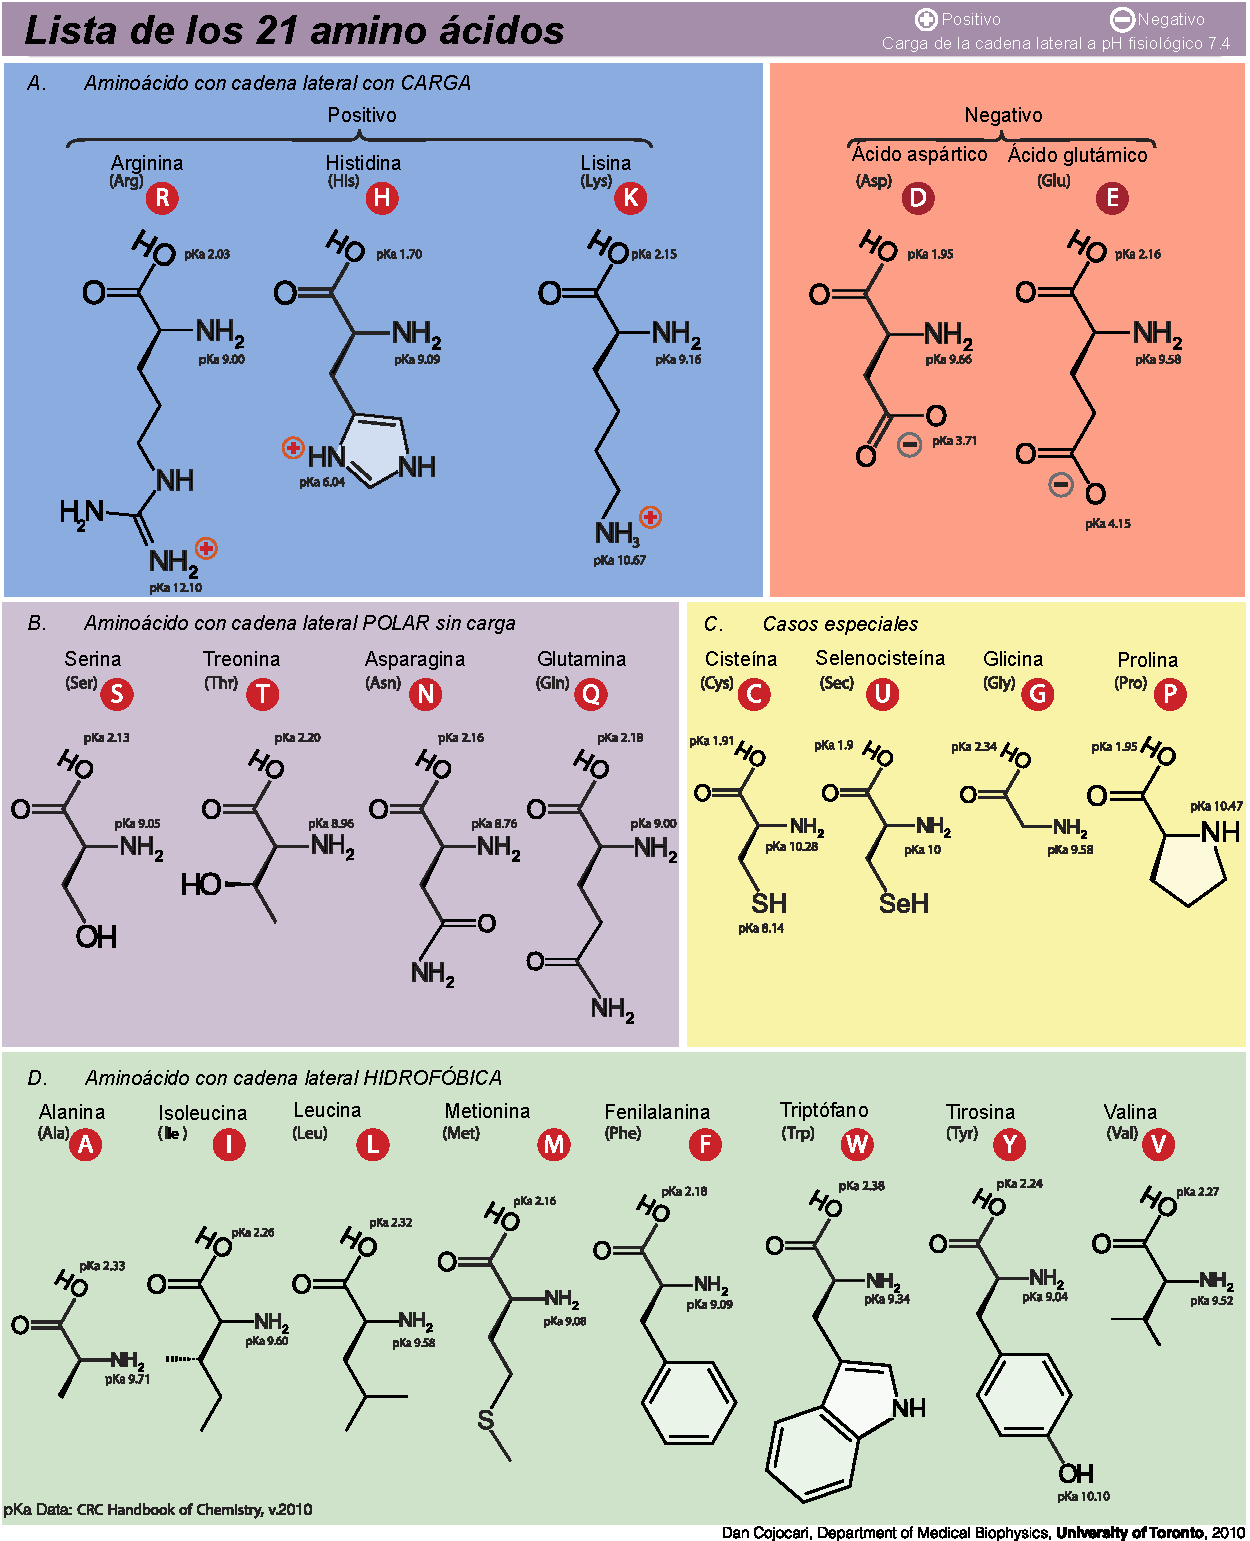
\includegraphics[width=1\linewidth, height=0.99\textheight, keepaspectratio]{fig/04_anexos/tabla_aa.pdf} 
\caption[]{Lista de los 21 amino ácidos, estructura química, código de letras, agrupados por propiedades fisicoquímicas. Figura adaptada por Dancojocari bajo \textit{Creative Commons} (CC BY-SA 3.0 - \url{https://commons.wikimedia.org/wiki/File:Amino_Acids.svg}).}
        \index{tabla_aa}
    \label{tab:tabla_aa}
\end{figure}
%%%%%%%%%%%%%%%%%%%%%%% Fin %%%%%%%%%%%%%%%%%%%%%%%%

\end{appendix}